\section{Poiseuille flow with ring-molecules}
For the Poiseuille flow simulation, two stationary walls were placed on opposite sides of the domain, and a constant body force $F_{body} = 0.3$ was applied to all non-wall particles. The system contained $10$ ring molecules (each with 9 particles of type A) alongside fluid particles. Bond parameters were $K_S = 100$ and $r_S = 0.3$.

\subsection{Flow Profile Analysis}
The velocity profile in Figure \ref{fig:poiseuille} shows the characteristic parabolic shape expected for Poiseuille flow, with maximum velocity in the center of the channel and zero velocity at the walls. This confirms the correct implementation of the body force and wall boundary conditions.

\subsection{Molecule Distribution and Evolution}
The ring molecules show a distinct distribution pattern across the channel:
\begin{enumerate}
	\item Initially randomly distributed, the rings gradually migrate toward the center of the channel over time.
	\item The molecule distribution histogram shows higher concentrations near the center and decreased presence near the walls.
	\item The rings appear to maintain their circular structure throughout the simulation, showing the effectiveness of the bond implementation.
\end{enumerate}

The migration of ring molecules toward the center is a phenomenon known as "cross-stream migration" or "tubular pinch effect." This effect has been observed in both simulations and experiments of flowing suspensions. The primary reason for this migration is the balance between:
\begin{enumerate}
	\item Wall-induced migration: The interaction with walls creates an effective repulsive force pushing particles away from the walls.
	\item Shear-induced migration: The non-uniform shear rate across the channel (highest near walls, lowest at center in Poiseuille flow) creates a driving force that moves particles from high-shear to low-shear regions.
\end{enumerate}
This effect is particularly pronounced for extended structures like our ring molecules, as they experience different shear forces across their structure when oriented obliquely to the flow. The resulting hydrodynamic lift pushes them toward the center of the channel where the shear rate is minimal.
Literature on the subject (e.g., Fedosov et al., "Cross-stream migration of deformable particles in microfluidic channels") confirms this behavior for various particle shapes in pressure-driven flows.

\begin{figure}[H]
	\begin{center}
		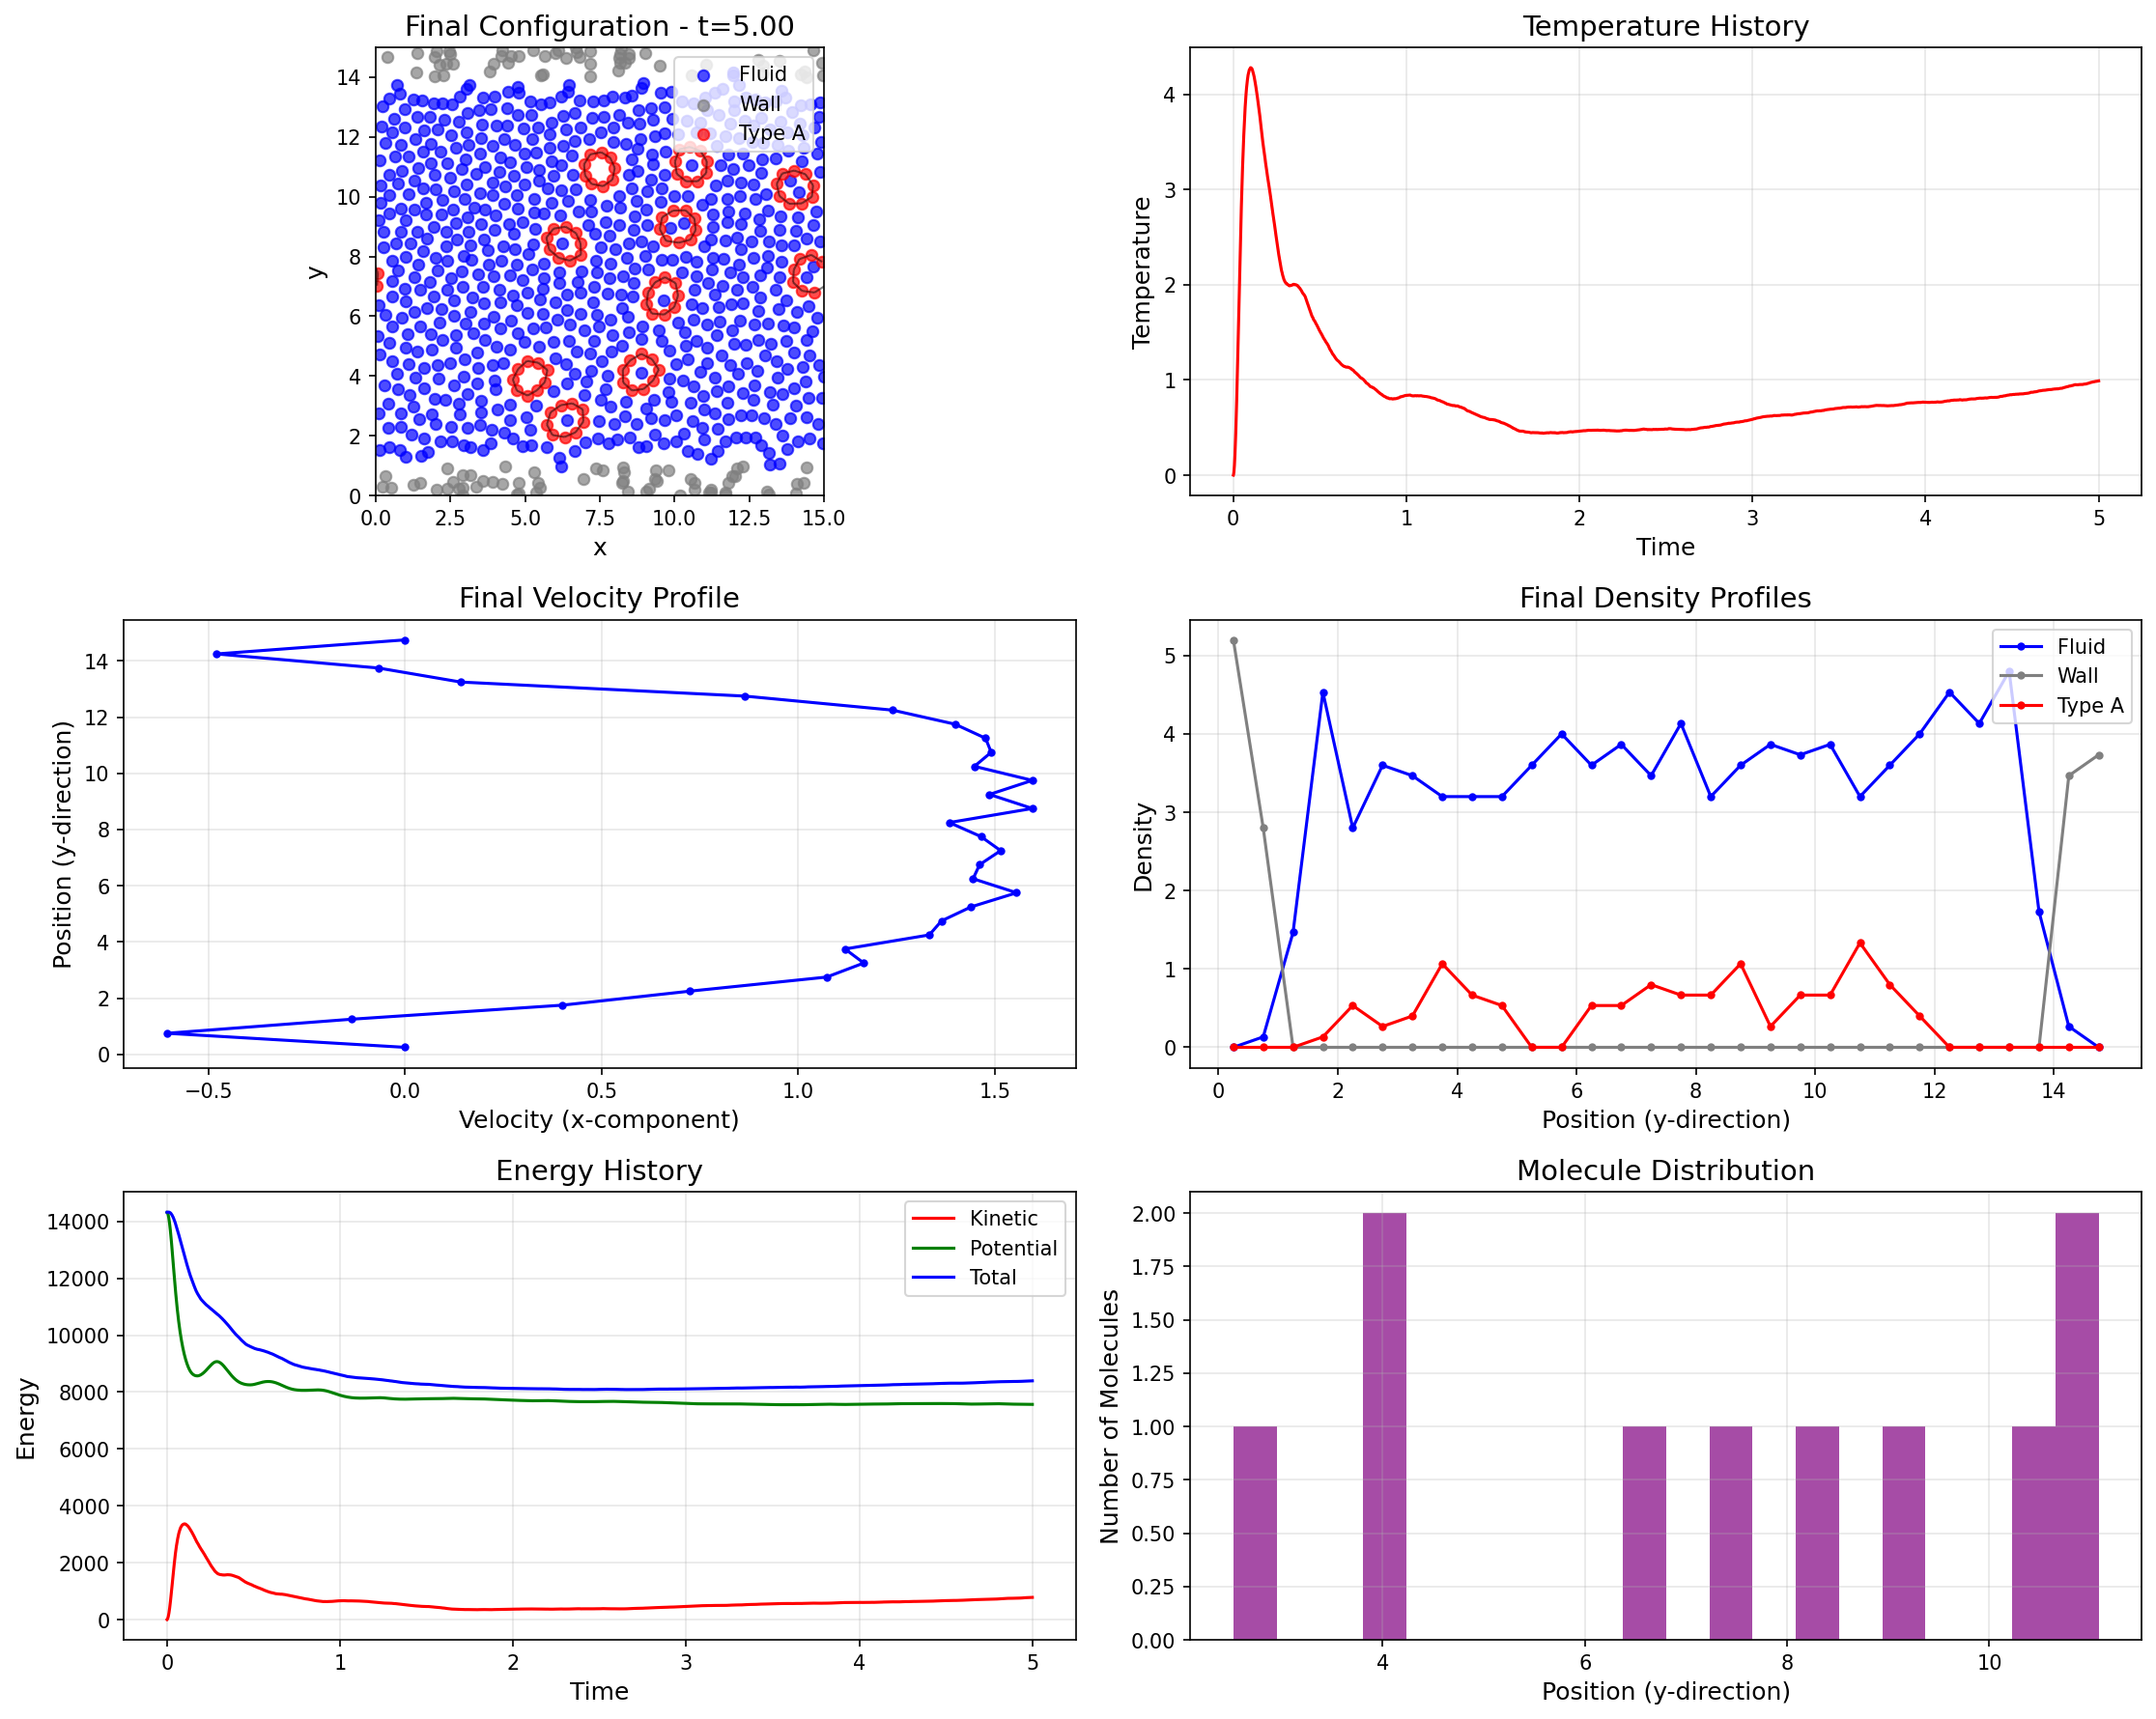
\includegraphics[width=0.95\textwidth]{figures/poiseuille_vis_final.png}
	\end{center}
	\caption{Poiseuille flow with $dt=0.001$ with $5000$ steps}\label{fig:poiseuille}
\end{figure}

\section*{Conclusion}
The DPD simulations successfully captured the expected behaviors of both Couette and Poiseuille flows. The implementation of chain and ring molecules demonstrated the capability of DPD to model complex fluids with structured components.
Key findings include:
\begin{enumerate}
	\item The DPD thermostat effectively maintained system temperature around the desired value.
	\item Chain molecules in Couette flow aligned with the flow direction and showed some level of aggregation.
	\item Ring molecules in Poiseuille flow exhibited cross-stream migration toward the center of the channel, consistent with theoretical predictions and experimental observations.
\end{enumerate}
These simulations illustrate the power of DPD as a mesoscopic simulation method that can capture complex phenomena at the interface between molecular and continuum scales. The soft repulsive potentials and momentum-conserving thermostat make it particularly suitable for simulating soft matter and complex fluids.
